%2019-09-14
\documentclass[compress,xcolor=dvipsnames]{beamer}
\usepackage{tikz,xstring,ifthen}
\usetikzlibrary{decorations.pathreplacing}
%???\usepackage{etex}
\usepackage{tabularx}
\usepackage{times}
\usepackage{pifont}
\usepackage{soul}
\usepackage[nomessages]{fp}

% Uniform random wiggly line of horizontal and vertical steps from (#1,#2) to (#3,#4) in #5 steps. Notice, #3>=#1 and #4>=#2 required. Apply in a tikz environment. To avoid rounding errors, make sure the ratio of horizontal and vertical distance divides #5 into integers. E.g, from (0,1.5) to (5,5) the ratio is 5:3.5, that is 10:7, so the number of steps should be a multiple of 17: \lppwl{0}{1.5}{5}{5}{34} .
% Optional argument in []: color (or anything else passed to draw[.]): \lppwl[green]{0}{1.5}{5}{5}{34}.
% Notice, due to this color is #1 and number options are #2...#6 in the code.
\newcounter{usedm}
\newcounter{usedn}
\newcommand*{\lppwl}[6][]{

% The number of right steps
 \FPeval{\m}{round(#6*(#4-#2)/(#4+#5-#2-#3),0)}

% The number of up steps
 \FPeval{\n}{round(#6*(#5-#3)/(#4+#5-#2-#3),0)}

% The length of steps
 \FPeval{\stlength}{(#4+#5-#2-#3)/#6}

% Initialize used steps
 \setcounter{usedm}{0}
 \setcounter{usedn}{0}
 
 \foreach\i in{1,...,{#6}}{
 % random is a number 0...1. Can also add seed with \FPseed{integer}.
  \FPrandom{\x}

% Compare with \usedm and \usedn.
  \FPeval{\y}{(\m-\theusedm)/(\m+\n-\theusedm-\theusedn)}

% Where are we?
  \FPeval{\startx}{#2+(\theusedm)*\stlength}
  \FPeval{\starty}{#3+(\theusedn)*\stlength}

% Need to use length for real comparison
  \ifthenelse{\lengthtest{\x pt > \y pt}}{
   \FPset{\endx}{\startx}
   \FPadd{\endy}{\starty}{\stlength}
   \stepcounter{usedn}
  }
  {
   \FPadd{\endx}{\startx}{\stlength}
   \FPset{\endy}{\starty}
   \stepcounter{usedm}
  }
  \draw[#1](\startx,\starty) -- (\endx,\endy);
 }
}

% Simple random walk. Starts at (#1,#2), in horizontal steps #3, vertical steps #4 + drift #5, #6 number of times. []is optional for draw.
\newcounter{ups}
\newcommand*{\srw}[7][]{
 
 \setcounter{ups}{0}
 \foreach\i in{1,...,{#7}}{
 % random is a number 0...1. Can also add seed with \FPseed{integer}.
  \FPrandom{\x}

  \FPeval{\startx}{(#2)+(\i-1)*(#4)}
  \FPeval{\starty}{(#3)+(2*\theups-\i+1)*#5+(i-1)*(#6)}
% Need to use length for real comparison
  \ifthenelse{\lengthtest{\x pt > 0.5 pt}}{
   \stepcounter{ups}
  }
  {
  }
  \FPeval{\endx}{(#2)+\i*(#4)}
  \FPeval{\endy}{(#3)+(2*\theups-\i)*#5+i*(#6)}
  \draw[#1](\startx,\starty) -- (\endx,\endy);
 }
}

\renewcommand\tabularxcolumn[1]{m{#1}}
\newcommand*{\Zp}{\mathbb Z_{\ge0}}
\newcommand*{\Zb}{\mathbb Z}
%\newcommand*{\ga}{\gamma}
\newcommand*{\om}{\omega}
\newcommand*{\vr}{\varrho}
\newcommand*{\la}{\lambda}
%\newcommand*{\un}{\underline}
%\newcommand*{\Ev}{{\bf E}}
\newcommand*{\Pv}{{\mathbb P}}
%\newcommand*{\dd}[1]{\frac{\text{d}}{\text{d}{#1}}}
%\newcommand*{\di}{\text{d}}
%\newcommand*{\pp}[1]{\frac\partial{\partial{#1}}}
%\newcommand*{\ppp}[1]{\frac{\partial^2}{\partial{#1}^2}}
%\newcommand*{\e}[1]{\text{\rm e}^{#1}}

%\newcounter{z}
%\newcounter{za}
%\newcounter{zb}
%\newcounter{zc}
%\newcounter{zd}
%\newcounter{ha}
%\newcounter{hb}
%\newcounter{hd}
%\newcounter{cga}
%\newcounter{cgb}
%\newcounter{cgc}
%\newcounter{cgab}
%\newcounter{cgbc}

%\newcount\x
%\newcount\xa
%\newcount\xb
%\newcount\xc
%\newcount\xd
%\newcount\xe

\useoutertheme{split}
\usecolortheme{dolphin}

\setbeamertemplate{navigation symbols}{}
\setbeamertemplate{footline}{}

\setbeamercolor{palette primary}{use=structure,bg=structure.fg!70!black,fg=white}
\setbeamercolor{subtitle}{fg=Orange}

\setbeamercolor{expl}{fg=YellowOrange}
\newcommand*{\expl}[1]{{\usebeamercolor[fg]{expl}#1}}
\setbeamercolor{blackk}{fg=Black}
\newcommand*{\blackk}[1]{{\usebeamercolor[fg]{blackk}#1}}
\setbeamercolor{gr}{fg=Gray}
\newcommand*{\gr}[1]{{\usebeamercolor[fg]{gr}#1}}
\setbeamercolor{olgr}{fg=OliveGreen}
\newcommand*{\olgr}[1]{{\usebeamercolor[fg]{olgr}#1}}
\setbeamercolor{cola}{fg=Black!\thecga!averagebackgroundcolor}
\newcommand*{\cola}[1]{{\usebeamercolor[fg]{cola}#1}}
\setbeamercolor{colb}{fg=Black!\thecgb!averagebackgroundcolor}
\newcommand*{\colb}[1]{{\usebeamercolor[fg]{colb}#1}}
\setbeamercolor{colc}{fg=Black!\thecgc!averagebackgroundcolor}
\newcommand*{\colc}[1]{{\usebeamercolor[fg]{colc}#1}}
\setbeamercolor{colab}{fg=Black!\thecgab!averagebackgroundcolor}
\newcommand*{\colab}[1]{{\usebeamercolor[fg]{colab}#1}}
\setbeamercolor{colbc}{fg=Black!\thecgbc!averagebackgroundcolor}
\newcommand*{\colbc}[1]{{\usebeamercolor[fg]{colbc}#1}}

\title{
 Nonexistence of bi-infinite geodesics in exponential last passage percolation - a probabilistic way
}
\author{M\'arton Bal\'azs}
\subtitle{\small Joint with\\
 Ofer Busani and Timo Sepp\"al\"ainen}
\date{Large Scale Stochastic Dynamics\\
 Oberwolfach, 17 September, 2019.
}
\institute{University of Bristol}

\begin{document}

%\frame{\titlepage}
\begin{frame}[plain]
 \titlepage
\end{frame}

%szerkbodystart

\frame{\tableofcontents}

\section[LPP]{Last passage percolation}

\subsection{Geodesics}

\begin{frame}{Last passage percolation}
 \begin{itemize}
  \item Place \(\om_z\) i.i.d.\ Exp(1) for \(z\in\Zb^2\).
  \item The \structure{\emph{geodesic}} \(\pi_{x,y}\) from \(x\) to \(y\) is the a.s.\ unique heaviest up-right from \(x\) to \(y\).
  \item \(G_{x,y}=\sum_{z\in\pi_{x,y}}\om_z\) is its weight.
 \end{itemize}
 \begin{center}
  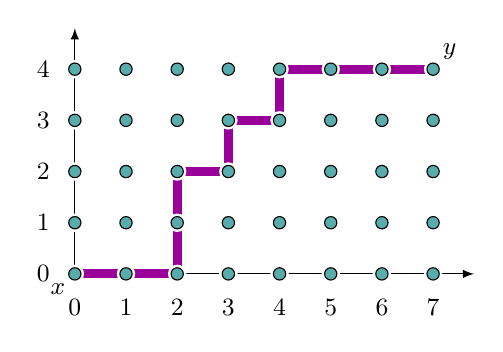
\begin{tikzpicture}[>=latex, scale=0.65]
   \definecolor{sussexg}{rgb}{0,0.5,0.5}
   \definecolor{sussexp}{rgb}{0.6,0,0.6} Uncomment for colorful version
   %\definecolor{sussexg}{gray}{0.7}
   %\definecolor{sussexp}{gray}{0.4} %comment out for colorful version
%AXES
   \draw[<->](0,4.8)--(0,0)--(7.8,0);
% PATH
   \draw[line width = 3.2 pt, color=sussexp](0,0)--(2,0)--(2,2)--(3,2)--(3,3)--(4,3)--(4,4)--(7,4);
% LATTICE
   \foreach \x in { 0,...,7}{
    \foreach \y in {0,...,4}{
     \fill[color=white] (\x,\y)circle(1.8mm);
% Above: Extra layer of circles to make the path disconnected at sites. Comment out for a different effect
     \draw[ fill=sussexg!65](\x,\y)circle(1.2mm);
    }
   }
%LABELS
   \foreach \x in {0,...,7}{\draw(\x, -0.3)node[below]{\small{$\x$}};}
   \foreach \x in {0,...,4}{\draw(-0.3, \x)node[left]{\small{$\x$}};}
   \draw(0,0)node[below left=]{\small{\(x\)}};
   \draw(7,4)node[above right=]{\small{\(y\)}};
  \end{tikzpicture}
 \end{center}
 \expl{Surface growth, TASEP, queuing\dots}
\end{frame}

\begin{frame}{Bi-infinite geodesics}
 A bi-infinite up-right path is a \structure{\emph{bi-infinite geodesic}}, if any of its segments is itself a geodesic between the two endpoints.
 \begin{center}
  \begin{tikzpicture}[>=latex]
   \draw[->](4,0)--(4,4);
   \draw[->](0,2)--(8,2);
   \only<1>{
    \lppwl{0}{0.2}{2}{1.2}{60}
    \lppwl{7}{3.2}{8}{3.5}{26}
    \draw(4,2.7)node[anchor=west]{\small{\(\pi_{\phantom{x,y}}\)}};
   }
   \FPseed=0
   \lppwl[blue,thick]{2}{1.2}{7}{3.2}{140}
   \only<2>{
    \draw(4,2.7)node[anchor=west]{\structure{\small{\(\pi_{x,y}\)}}};
    \draw(2,1.2)node[below left=]{\small{\(x\)}};
    \draw(7,3.2)node[above right=]{\small{\(y\)}};
   }
  \end{tikzpicture}
 \end{center}
\end{frame}

\begin{frame}{Bi-infinite geodesics}
 Trivial bi-infinite geodesics:
 \begin{center}
  \begin{tikzpicture}[>=latex]
   \draw[->](4,0)--(4,4);
   \draw[->](0,2)--(8,2);
   \only<1>{
    \draw(0,3)--(8,3);
   }
   \only<2>{
    \draw(5.5,0)--(5.5,4);
   }
  \end{tikzpicture}
 \end{center}
\end{frame}

\section{The result}

\begin{frame}{The result}
 \begin{theorem}
  A.s., there are no non-trivial bi-infinite geodesics.
 \end{theorem}
 \begin{itemize}
  \item<2-> Question raised in first passage percolation (FPP) to \expl{Kesten} by \expl{Furstenberg} in '86.
  \item<3-> \expl{Licea, Newman '96}: almost no direction with bi-infinite geodesics in FPP.
  \item<4-> \st{Almost} \(\to\) in any fixed direction: \expl{Ahlberg, Hoffman '16}; \expl{Damron, Hanson '17} (\structure{FPP}); \expl{Georgiou, Rassoul-Agha, Sepp\"al\"ainen '17} (\structure{LPP}). The problem is, uniqueness of geodesics is still needed.
  \item<5-> Full result by \expl{Basu, Hoffman, Sly '18}, using estimates from integrable probability.
  \item<6-> We only need a bit of random walks, queuing, couplings.
 \end{itemize}
\end{frame}

\section{Tools}

\subsection{New boundary}

\begin{frame}{1. Increments as new boundary}
 \begin{center}
  \begin{tikzpicture}[>=latex]
   \filldraw(0,0) circle (1.5pt);
   \draw(0,0)node[below left=]{\small{\(a\)}};
   \filldraw(8,4) circle (1.5pt);
   \draw(8,4)node[above right=]{\small{\(y\)}};

   \only<1>{
    \FPseed=0
    \lppwl{0}{0}{4}{1}{10}
    \lppwl{4}{1}{4.5}{1.5}{2}
    \lppwl{4.5}{1.5}{5}{2}{2}
    \lppwl{4}{1}{5.5}{1}{3}
    \lppwl{5.5}{1}{5.5}{2}{2}
    \filldraw(5,2) circle (1.5pt);
    \filldraw(5.5,2) circle (1.5pt);
    \draw(5,2)node[above]{\small{\(x-e_1\)}};
    \draw(5.5,2)node[below right=]{\small{\(x\)}};
    \draw[blue,very thick](5.1,2)--(5.4,2);
   }

   \only<2>{
    \lppwl{0}{0}{3}{1.5}{9}
    \lppwl{3}{1.5}{3.5}{2}{2}
    \lppwl{3.5}{2}{4}{2.5}{2}
    \lppwl{3}{1.5}{3.5}{2.5}{3}
    \lppwl{3.5}{2.5}{4}{3}{2}
    \filldraw(4,2.5) circle (1.5pt);
    \filldraw(4,3) circle (1.5pt);
    \draw(4,3)node[right]{\small{\(x\)}};
    \draw(4,2.5)node[right]{\small{\(x-e_2\)}};
    \draw[blue,very thick](4,2.6)--(4,2.9);
   }

   \only<3->{
    \filldraw(4,2) circle (1.5pt);
    \foreach\i in {4.5,5,...,8}{
     \filldraw(\i,2) circle (1.5pt);
     \draw[blue,very thick](\i-0.4,2)--(\i-0.1,2);
    }
    \foreach\j in {2.5,3,...,4}{
     \filldraw(4,\j) circle (1.5pt);
     \draw[blue,very thick](4,\j-0.4)--(4,\j-0.1);
    }
   }
   \only<4->{
    \FPseed=0
    \lppwl{4}{3}{8}{4}{10}
   }
   \only<5->{
    \FPseed=0
    \lppwl[red,thick]{4}{3}{8}{4}{10}
   }
   \only<4,5>{
    \lppwl{0}{0}{4}{3}{14}
   }
   \only<6->{
    \draw(4,2)--(4,3);
   }
   
  \end{tikzpicture}
 \end{center}
 \[
  I_x=G_{a,x}-G_{a,x-e_1}\qquad\uncover<2->{
   J_x=G_{a,x}-G_{a,x-e_2}
  }
 \]
 \uncover<6->{
  \structure{\(\leadsto\)} Act as boundary weights for a smaller, embedded model.
 }
\end{frame}

\subsection{Crossing}

\begin{frame}{2. Crossing lemma}
 Let \alert{\(a\)} be North-West of \olgr{\(b\)}.
 \begin{center}
  \begin{tikzpicture}[>=latex]
   \filldraw[red](0,1)node[above left=]{\small{\(a\)}}circle (1.5pt);
   \filldraw[olive](1,0)node[below right=]{\small{\(b\)}}circle (1.5pt);
   \FPseed=0
   \lppwl[red]{0}{1}{1}{2}{4}
   \draw[red](4,2.5)--(2.5,2.5)--(2.5,2)--(1,2)--(1,2.5)--(2,2.5)--(2,3)--(4,3);
   \lppwl[olive]{1}{0}{3}{1}{6}
   \draw[olive](4,2.5)--(4,2)--(3.5,2)--(3.5,1)--(3,1)--(3,2.98)--(4,2.98);
   \filldraw(3,2.5)node[below left=]{\small{\(u\)}}circle(1.5pt);
   \filldraw(4,2.5)circle (1.5pt);
   \filldraw(4,3)circle (1.5pt);
   \draw(4,3)node[right]{\small{\(x\)}};
   \draw(4,2.5)node[right]{\small{\(x-e_2\)}};
   \draw[blue,very thick](4,2.6)--(4,2.9);

  \end{tikzpicture}
 \end{center}
 \[
  \begin{aligned}
   \uncover<2->{
    G_{a,x}&\ge G_{a,u}+G_{u,x},&\qquad G_{b,x-e_2}&\ge G_{b,u}+G_{u,x-e_2},
   }\\
   \uncover<3->{
    G_{a,x-e_2}&=G_{a,u}+G_{u,x-e_2},&\qquad G_{b,x}&=G_{b,u}+G_{u,x}.
   }
  \end{aligned}
 \]
 \uncover<4->{
  \[
   \alert{J^{(a)}_x}=G_{a,x}-G_{a,x-e_2}\ge G_{u,x}-G_{u,x-e_2}\ge G_{b,x}-G_{b,x-e_2}=\olgr{J^{(b)}_x}.
  \]
 }
 \uncover<5->{
  Similarly, \(\alert{I^{(a)}_x}\le\olgr{I^{(b)}_x}\).
 }
\end{frame}

\subsection{Stationarity}

\begin{frame}{3. Stationary LPP}
 \uncover<2->{
  Replace the boundary to \begin{tikzpicture}\draw[olive,very thick](0,0)--(0,0.3);\end{tikzpicture} \olgr{\(\sim\text{Exp}(\vr)\)}, \begin{tikzpicture}\draw[olive,very thick](0,0)--(0.3,0);\end{tikzpicture} \olgr{\(\sim\text{Exp}(1-\vr)\)} independent.
 }
 \begin{center}
  \begin{tikzpicture}[>=latex]
   \filldraw(0,0) circle (1.5pt);
   \draw(0,0)node[below left=]{\small{\(a\)}};
   \filldraw(8,4) circle (1.5pt);
   \draw(8,4)node[above right=]{\small{\(y\)}};

   \filldraw(4,2) circle (1.5pt);
   \foreach\i in {4.5,5,...,8}{
    \filldraw(\i,2) circle (1.5pt);
    \draw[blue,very thick](\i-0.4,2)--(\i-0.1,2);
   }
   \foreach\j in {2.5,3,...,4}{
    \filldraw(4,\j) circle (1.5pt);
    \draw[blue,very thick](4,\j-0.4)--(4,\j-0.1);
   }
   \FPseed=0
   \lppwl{4}{3}{8}{4}{10}
   \only<3->{
    \FPseed=0
    \lppwl[red,thick]{4}{3}{8}{4}{10}
   }
   \lppwl{0}{0}{4}{3}{14}

   \only<2->{
    \foreach\i in {0.5,1,...,8}{
     \filldraw(\i,0) circle (1.5pt);
     \draw[olive,very thick](\i-0.4,0)--(\i-0.1,0);
    }
    \foreach\j in {0.5,1,...,4}{
     \filldraw(0,\j) circle (1.5pt);
     \draw[olive,very thick](0,\j-0.4)--(0,\j-0.1);
    }
   }
   
  \end{tikzpicture}
 \end{center}
 \[
  I_x=G_{a,x}-G_{a,x-e_1}\qquad J_x=G_{a,x}-G_{a,x-e_2}
 \]
 \uncover<2->{
  Then \structure{\(J_x\) \(\sim\text{Exp}(\vr)\)}, \structure{\(I_x\) \(\sim\text{Exp}(1-\vr)\)}, independent.
 }

 \uncover<3->{
  \alert{\emph{The embedded model has the same structure.}}
 }
\end{frame}

\begin{frame}{3. Stationary LPP}
 Replace the boundary to \begin{tikzpicture}\draw[olive,very thick](0,0)--(0,0.3);\end{tikzpicture} \olgr{\(\sim\text{Exp}(\vr)\)}, \begin{tikzpicture}\draw[olive,very thick](0,0)--(0.3,0);\end{tikzpicture} \olgr{\(\sim\text{Exp}(1-\vr)\)} independent.
 \begin{center}
  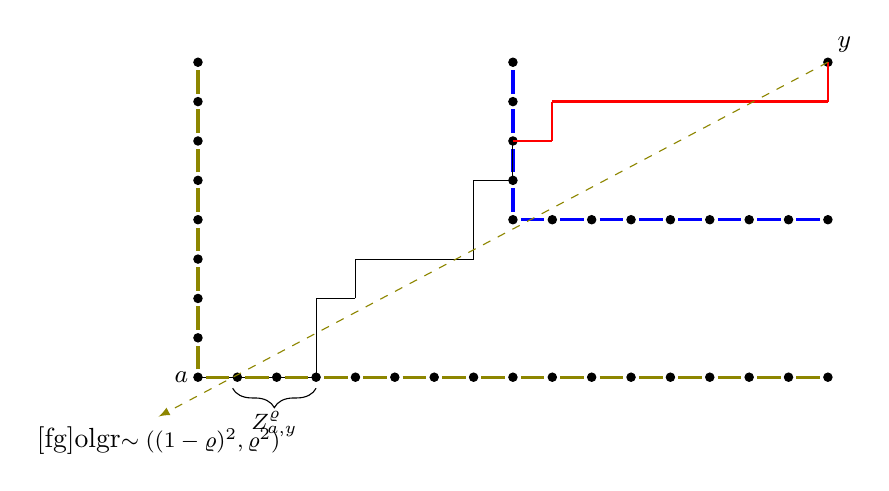
\begin{tikzpicture}[>=latex]
   \filldraw(0,0) circle (1.5pt);
   \draw(0,0)node[left]{\small{\(a\)}};
   \filldraw(8,4) circle (1.5pt);
   \draw(8,4)node[above right=]{\small{\(y\)}};

   \filldraw(4,2) circle (1.5pt);
   \foreach\i in {4.5,5,...,8}{
    \filldraw(\i,2) circle (1.5pt);
    \draw[blue,very thick](\i-0.4,2)--(\i-0.1,2);
   }
   \foreach\j in {2.5,3,...,4}{
    \filldraw(4,\j) circle (1.5pt);
    \draw[blue,very thick](4,\j-0.4)--(4,\j-0.1);
   }
   \FPseed=0
   \lppwl{4}{3}{8}{4}{10}
   \FPseed=0
   \lppwl[red,thick]{4}{3}{8}{4}{10}
   \lppwl{0}{0}{4}{3}{14}

   \foreach\i in {0.5,1,...,8}{
    \filldraw(\i,0) circle (1.5pt);
    \draw[olive,very thick](\i-0.4,0)--(\i-0.1,0);
   }
   \foreach\j in {0.5,1,...,4}{
    \filldraw(0,\j) circle (1.5pt);
    \draw[olive,very thick](0,\j-0.4)--(0,\j-0.1);
   }
   \draw[->,dashed,olive](8,4)--(-0.5,-0.5);
   \draw(-0.5,-0.5)node[below]{\olgr{\footnotesize{\(\sim((1-\vr)^2,\vr^2)\)}}};
   \draw [decorate,decoration={brace,amplitude=7pt,mirror},yshift=-4pt,xshift=0pt](0.44,0)--(1.5,0)node[black,midway,yshift=-13pt]{\footnotesize\(Z^\vr_{a,y}\)};
  \end{tikzpicture}
 \end{center}
 \expl{B., Cator, Sepp\"al\"ainen '06}: \(\Pv\{|Z^\vr_{a,y}|\ge\ell\}\le\text{box}^2/\ell^3\), \emph{good directional control}.
\end{frame}

\section{Proof}

\begin{frame}{Proof}
 Take larger and larger boxes and show that geodesics avoid more and more the origin when crossing from one side to the other (\expl{Newman '95}).
 \begin{enumerate}
  \item<2->Close to vertical and horizontal all semi-infinite geodesics become trivial.
  \item<3->Otherwise, geodesics don't like to turn too much.
  \item<4->We are left with roughly diagonal ones, show that they fluctuate too much.
 \end{enumerate}
 \begin{center}
  \begin{tikzpicture}[>=latex]
   \draw(0,0)--(4,0)--(4,4)--(0,4)--(0,0);
   \draw[dotted](2,0)--(2,4);
   \draw[dotted](0,2)--(4,2);
   \only<2>{
    \draw[thick,red](0,2)--(4,2);
   }
   \only<3>{
    \lppwl[thick,red]{0}{1}{2}{2}{30}
    \lppwl[thick,red]{2}{2}{3}{4}{30}
    \draw[red,dashed](0,1)--(3,4);
    \draw(3.2,3)node{\alert{\Huge{\ding{55}}}};
   }
   \only<4>{
    \lppwl[thick,red]{0}{1}{4}{3}{60}
   }
  \end{tikzpicture}
 \end{center}
\end{frame}

\subsection[Flat]{When it's too flat}

\begin{frame}{1. When it's too flat}
 \begin{center}
  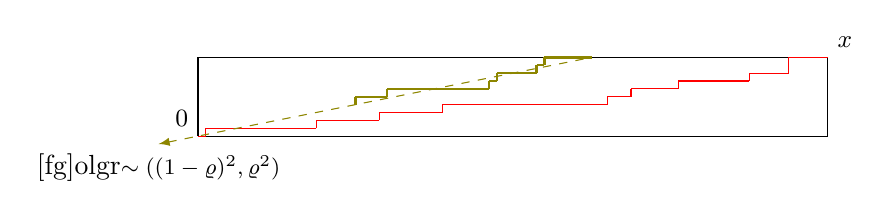
\begin{tikzpicture}[>=latex]
   \draw(0,0)--(8,0)--(8,1)--(0,1)--(0,0);
   \lppwl[red]{0}{0}{8}{1}{90}
   \lppwl[olive,thick]{2}{0.4}{5}{1}{36}
   \draw[olive,dashed,<-](-0.5,-0.1)--(5,1);
   \draw(-0.5,-0.1)node[below]{\olgr{\footnotesize{\(\sim((1-\vr)^2,\vr^2)\)}}};
   \draw(0,0)node[above left=]{\small{\(0\)}};
   \draw(8,1)node[above right=]{\small{\(x\)}};
  \end{tikzpicture}
 \end{center}
 Take \olgr{\(\vr\)} small, but not too small compared to \(x\), so that with large probability the \olgr{green stationary path} exits on the left of \(x\) (use the shape function here).
 \[
  G_{0,x}-G_{e_2,x}=\hat J_{e_2}\ge\olgr{\hat J^\vr_{e_1}\sim\text{Exp}(\vr)},
 \]
 and can take \(\vr\to0\) as the box flattens with \(x\to\infty\). So, it's never worth leaving from \(e_2\) compared from 0.
\end{frame}

\subsection[No turns]{No sharp turns please}

\begin{frame}{2. No sharp turns please}
 \begin{center}
  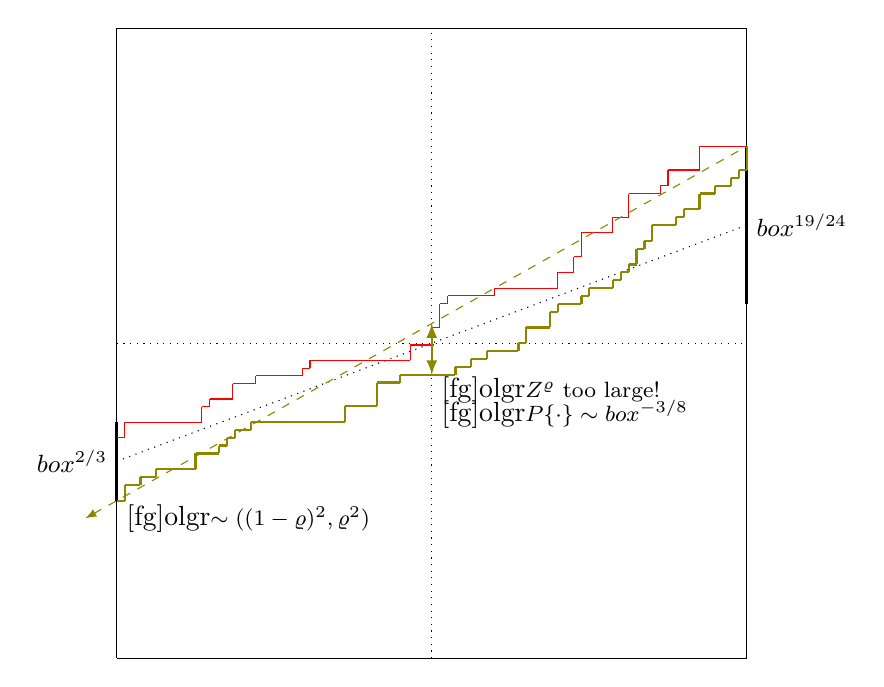
\begin{tikzpicture}[>=latex]
   \draw(0,0)--(8,0)--(8,8)--(0,8)--(0,0);
   \draw[dotted](0,4)--(8,4);
   \draw[dotted](4,0)--(4,8);
   \draw[dotted](0,2.5)--(8,5.5);
   \draw[very thick](0,2)--(0,3);
   \draw[very thick](8,4.5)--(8,6.5);
   \draw(0,2.5)node[left]{\small{\(\text{box}^{2/3}\)}};
   \draw(8,5.5)node[right]{\small{\(\text{box}^{19/24}\)}};
   \FPseed=0
   \lppwl[red]{0}{2.8}{4}{4}{53}
   \lppwl[red]{4}{4}{8}{6.5}{65}
   \draw[olive,dashed,<-](-0.4,1.775)--(8,6.5);
   \draw(0,1.775)node[right]{\olgr{\footnotesize{\(\sim((1-\vr)^2,\vr^2)\)}}};
   \lppwl[olive,thick]{0}{2}{4.1}{3.6}{57}
   \lppwl[olive,thick]{4.1}{3.6}{8}{6.5}{68}
   \draw[thick,olive,<->](4,3.6)--(4,4.25);
   \draw(4,3.7)node[below right=]{\olgr{\footnotesize{\(Z^\vr\) too large!}}};
   \draw(4,3.4)node[below right=]{\olgr{\footnotesize{\(\Pv\{\cdot\}\sim\text{box}^{-3/8}\)}}};
  \end{tikzpicture}
 \end{center}
\end{frame}

\subsection[Diagonal]{The diagonal case}

\begin{frame}{3. The diagonal case: the attack of the geodesics}
 \begin{center}
  \begin{tikzpicture}[>=latex]
   \draw(0,0)--(8,0)--(8,8)--(0,8)--(0,0);
   \draw[dotted](0,4)--(8,4);
   \draw[dotted](4,0)--(4,8);
   \draw[dotted](0,2.5)--(8,5.5);
   \draw[very thick](0,2)--(0,3);
   \draw[very thick](4,3.7)--(4,4.3);
   \draw[very thick](8,4.5)--(8,6.5);
   \draw(0,2.5)node[left]{\small{\(\text{box}^{2/3}\)}};
   \draw(4,3.5)node[right]{\small{\(\text{box}^{2/3}\)}};
   \draw(8,5.5)node[right]{\small{\(\text{box}^{19/24}\)}};
   \FPseed=0
   \lppwl[red]{0}{2.8}{8}{5.2}{100}

   \draw[olive,dashed,<-](-0.4,1.77)--(4,4.3);
   \lppwl[olive,thick]{0}{2}{1}{2.6}{16}

   \draw[olive,dashed,->](4,3.7)--(8.4,6.78);
   \lppwl[olive,thick]{7}{5.8}{8}{6.5}{17}

   \draw[blue,dashed,<-](-0.4,2.93)--(4,3.7);
   \lppwl[blue,thick]{0}{3}{1}{3.3}{13}

   \draw[blue,dashed,->](4,4.3)--(8.4,4.52);
   \lppwl[blue,thick]{7}{4.3}{8}{4.5}{12}
  \end{tikzpicture}
 \end{center}
\end{frame}

\begin{frame}{3. The diagonal case: the attack of the geodesics}
 With high probability, \(\forall u,\,x,\,v\):
 \begin{center}
  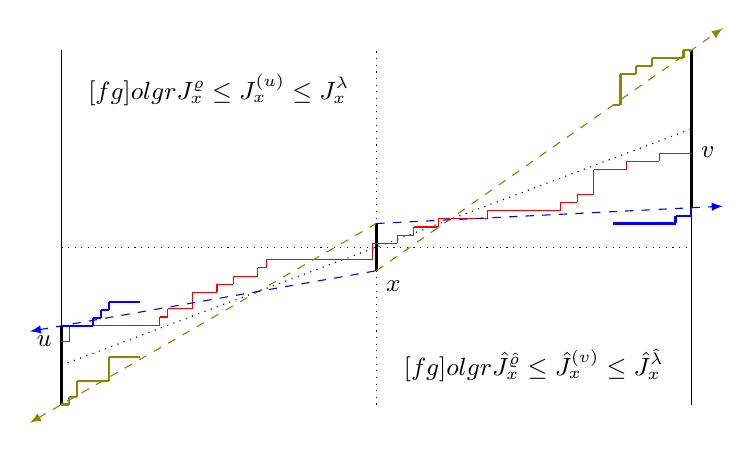
\begin{tikzpicture}[>=latex]
   \draw(0,6.5)--(0,2);
   \draw(8,2)--(8,6.5);
   \draw[dotted](0,4)--(8,4);
   \draw[dotted](4,2)--(4,6.5);
   \draw[dotted](0,2.5)--(8,5.5);
   \draw[very thick](0,2)--(0,3);
   \draw[very thick](4,3.7)--(4,4.3);
   \draw[very thick](8,4.5)--(8,6.5);
   \draw(0,2.8)node[left]{\small{\(u\)}};
   \draw(4,3.5)node[right]{\small{\(x\)}};
   \draw(8,5.2)node[right]{\small{\(v\)}};
   \FPseed=0
   \lppwl[red]{0}{2.8}{8}{5.2}{100}

   \draw[olive,dashed,<-](-0.4,1.77)--(4,4.3);
   \lppwl[olive,thick]{0}{2}{1}{2.6}{16}

   \draw[olive,dashed,->](4,3.7)--(8.4,6.78);
   \lppwl[olive,thick]{7}{5.8}{8}{6.5}{17}

   \draw[blue,dashed,<-](-0.4,2.93)--(4,3.7);
   \lppwl[blue,thick]{0}{3}{1}{3.3}{13}

   \draw[blue,dashed,->](4,4.3)--(8.4,4.52);
   \lppwl[blue,thick]{7}{4.3}{8}{4.5}{12}

   \draw(2,6)node{\small{\(\olgr{J^\vr_x}\le J^{(u)}_x\le\structure{J^\la_x}\)}};

   \draw(6,2.5)node{\small{\(\olgr{\hat J^{\hat\vr}_x}\le\hat J^{(v)}_x\le\structure{\hat J^{\hat\la}_x}\)}};
  \end{tikzpicture}
 \end{center}
 \begin{itemize}
  \item<2->The \alert{red geodesic} crosses where \(\sum_{j=0}^x(J^{(u)}_j-\hat J^{(v)}_j)\) is maximal.
  \item<3->The bounds \(\olgr{J_j^\vr}-\structure{\hat J^{\hat\la}_j}\le J^{(u)}_j-\hat J^{(v)}_j\le\structure{J^\la_j}-\olgr{\hat J^{\hat\vr}_j}\) are independent and nicely distributed.
 \end{itemize}
\end{frame}

\begin{frame}{3. The diagonal case: the attack of the geodesics}
 With high probability, \(\forall u,\,x,\,v\):
 \begin{itemize}
  \item The \alert{red geodesic} crosses where \(\sum_{j=0}^x(J^{(u)}_j-\hat J^{(v)}_j)\) is maximal.
  \item The bounds \(\olgr{J_j^\vr}-\structure{\hat J^{\hat\la}_j}\le J^{(u)}_j-\hat J^{(v)}_j\le\structure{J^\la_j}-\olgr{\hat J^{\hat\vr}_j}\) are independent and nicely distributed.
 \end{itemize}

 The problem boils down to whether a simple random walk minus drift reaches its maximum at 0. The answer is an asymptotic \emph{no}, the drift is beaten by the fluctuations.
 \begin{center}
  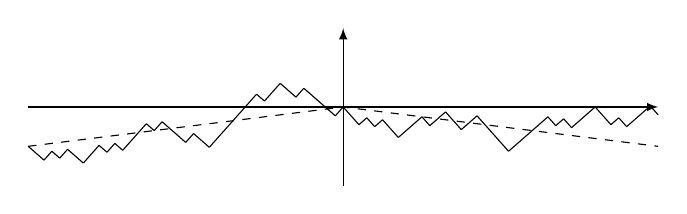
\begin{tikzpicture}[>=latex]
   \draw[->](0,2)--(8,2);
   \draw[->](4,1)--(4,3);
   \draw[dashed](0,1.5)--(4,2)--(8,1.5);
   \FPseed=1
   \srw{4}{2}{0.1}{0.1}{-0.0125}{40}
   \srw{4}{2}{-0.1}{0.1}{-0.0125}{40}
  \end{tikzpicture}
 \end{center}
 \(\Pv\{\cdot\}\sim\text{box}^{-2/5}\).
\end{frame}

\begin{frame}{So, the counting}
 \begin{itemize}
  \item Intervals on the left are of size \(\sim\text{box}^{2/3}\).
  \item Have \(\text{box}/\text{box}^{2/3}\sim\text{box}^{1/3}\) many of these.  
 \end{itemize}
 \structure{\(\leadsto\)} Union bound:
 \[
  \begin{aligned}
   \Pv\{\text{any geodesic crosses }0\}&\sim\text{box}^{1/3}\cdot\bigl(\text{box}^{-3/8}+\text{box}^{-2/5}\bigr)\\
   &=\text{box}^{-1/24}\to0.
  \end{aligned}
 \]
 \uncover<2->{
  These sharper, probabilistic estimates open up the way to further understanding of geodesics, with rather intuitive arguments.

  \begin{center}
   \structure{\emph{Thank you.}}
  \end{center}
 }
\end{frame}

%szerkbodyend

\end{document}
